\documentclass[]{book}
\usepackage{lmodern}
\usepackage{amssymb,amsmath}
\usepackage{ifxetex,ifluatex}
\usepackage{fixltx2e} % provides \textsubscript
\ifnum 0\ifxetex 1\fi\ifluatex 1\fi=0 % if pdftex
  \usepackage[T1]{fontenc}
  \usepackage[utf8]{inputenc}
\else % if luatex or xelatex
  \ifxetex
    \usepackage{mathspec}
  \else
    \usepackage{fontspec}
  \fi
  \defaultfontfeatures{Ligatures=TeX,Scale=MatchLowercase}
\fi
% use upquote if available, for straight quotes in verbatim environments
\IfFileExists{upquote.sty}{\usepackage{upquote}}{}
% use microtype if available
\IfFileExists{microtype.sty}{%
\usepackage{microtype}
\UseMicrotypeSet[protrusion]{basicmath} % disable protrusion for tt fonts
}{}
\usepackage{hyperref}
\hypersetup{unicode=true,
            pdftitle={Mind, Brain, Body},
            pdfauthor={Emily Towner},
            pdfborder={0 0 0},
            breaklinks=true}
\urlstyle{same}  % don't use monospace font for urls
\usepackage{natbib}
\bibliographystyle{apalike}
\usepackage{longtable,booktabs}
\usepackage{graphicx,grffile}
\makeatletter
\def\maxwidth{\ifdim\Gin@nat@width>\linewidth\linewidth\else\Gin@nat@width\fi}
\def\maxheight{\ifdim\Gin@nat@height>\textheight\textheight\else\Gin@nat@height\fi}
\makeatother
% Scale images if necessary, so that they will not overflow the page
% margins by default, and it is still possible to overwrite the defaults
% using explicit options in \includegraphics[width, height, ...]{}
\setkeys{Gin}{width=\maxwidth,height=\maxheight,keepaspectratio}
\IfFileExists{parskip.sty}{%
\usepackage{parskip}
}{% else
\setlength{\parindent}{0pt}
\setlength{\parskip}{6pt plus 2pt minus 1pt}
}
\setlength{\emergencystretch}{3em}  % prevent overfull lines
\providecommand{\tightlist}{%
  \setlength{\itemsep}{0pt}\setlength{\parskip}{0pt}}
\setcounter{secnumdepth}{5}
% Redefines (sub)paragraphs to behave more like sections
\ifx\paragraph\undefined\else
\let\oldparagraph\paragraph
\renewcommand{\paragraph}[1]{\oldparagraph{#1}\mbox{}}
\fi
\ifx\subparagraph\undefined\else
\let\oldsubparagraph\subparagraph
\renewcommand{\subparagraph}[1]{\oldsubparagraph{#1}\mbox{}}
\fi

%%% Use protect on footnotes to avoid problems with footnotes in titles
\let\rmarkdownfootnote\footnote%
\def\footnote{\protect\rmarkdownfootnote}

%%% Change title format to be more compact
\usepackage{titling}

% Create subtitle command for use in maketitle
\providecommand{\subtitle}[1]{
  \posttitle{
    \begin{center}\large#1\end{center}
    }
}

\setlength{\droptitle}{-2em}

  \title{Mind, Brain, Body}
    \pretitle{\vspace{\droptitle}\centering\huge}
  \posttitle{\par}
    \author{Emily Towner}
    \preauthor{\centering\large\emph}
  \postauthor{\par}
      \predate{\centering\large\emph}
  \postdate{\par}
    \date{2020-04-02}

\usepackage{booktabs}
\usepackage{amsthm}
\makeatletter
\def\thm@space@setup{%
  \thm@preskip=8pt plus 2pt minus 4pt
  \thm@postskip=\thm@preskip
}
\makeatother

\begin{document}
\maketitle

{
\setcounter{tocdepth}{1}
\tableofcontents
}
\hypertarget{introduction}{%
\chapter{Introduction}\label{introduction}}

The Mind, Brain, Body study looks at how early caregiving experiences influence the emotional, cognitive, and brain development, as well as physical health and wellness.

The study also explores how the bacteria that live inside us (the microbiome) are connected to the development of our brains and bodies.

\hypertarget{checklists}{%
\chapter{Checklists}\label{checklists}}

\begin{center}\rule{0.5\linewidth}{\linethickness}\end{center}

\hypertarget{initial-checklist}{%
\section{Initial Checklist}\label{initial-checklist}}

\textbf{Scheduling and Confirmation}

\begin{itemize}
\tightlist
\item
  Schedule lab session
\item
  Send confirmation email (in templates)

  \begin{itemize}
  \tightlist
  \item
    Attach \href{https://www.dropbox.com/s/3f9o2602kxfg54e/Mind_Brain_Body_Study_Next_Steps.pdf?dl=0}{Next Steps}
  \end{itemize}
\end{itemize}

\textbf{Enrollment}

\begin{itemize}
\tightlist
\item
  Create participant Dropbox folder using MBB\_template (delete blank README from newly created folder)
\item
  Enroll participant in Wave 1 on REDCap
\item
  Fill participant instrument on REDCap
\item
  Fill counterbalance order on REDCap (Checklist - Lab Session Child Instrument)
\item
  Print \href{https://paper.dropbox.com/doc/MBB-Lab-Session-Checklist-Child--AxSoiWlu0j1LQ~GQsuXI~DKpAg-h6fhBdxRjpAtpxDT5Vph1}{MBB Lab-Session Checklist-Child}
\item
  Print \href{https://paper.dropbox.com/doc/MBB-Lab-Session-Checklist-Parent--AxTlbCqV5ysM9LZxJpYPArWLAg-Rb5GOefE4nCOTTRpn84gv}{MBB Lab-Session Checklist-Parent}
\end{itemize}

\textbf{Calendar}

\begin{itemize}
\tightlist
\item
  Create MBB calendar event lab session and invite researchers
\item
  Create DBS calendar event (SAND calendar)
\item
  Create MBB calendar event lab session reminder 1 (email) (1 week prior)
\item
  Create MBB calendar event lab session reminder 2 (email and call) (3 days prior)
\item
  Create MBB calendar event to send home session reminder 1 (email) (1 week after lab session)
\item
  Create MBB calendar event to make home session reminder 1 (call) (8 days after lab session)
\item
  Create MBB calendar event to send home session reminder 2 (email) (10 days after lab session)
\item
  Create MBB calendar event to send home session reminder 3 email (14 days after lab session)
\end{itemize}

\textbf{Reminders}

\begin{itemize}
\tightlist
\item
  Send lab session reminder 1 email (in templates - attach next steps, consent/assent)
\item
  Send lab session reminder 2 email (in templates - attach previous and parking info)
\item
  Confirm participant

  \begin{itemize}
  \tightlist
  \item
    Preferably by phone
  \item
    Update lab session calendar status
  \end{itemize}
\end{itemize}

\begin{center}\rule{0.5\linewidth}{\linethickness}\end{center}

\hypertarget{pre-lab-session-checklist}{%
\section{Pre-Lab Session Checklist}\label{pre-lab-session-checklist}}

\hypertarget{lab-session-setup---1-day-prior}{%
\subsection{Lab Session Setup - 1 Day Prior}\label{lab-session-setup---1-day-prior}}

\begin{itemize}
\tightlist
\item
  Create participant manila folder
\item
  Print assent/consent forms (Check IRB expiration)

  \begin{itemize}
  \tightlist
  \item
    \href{https://www.dropbox.com/s/z729okdpqbvnbuc/Parent_consent.pdf?dl=0}{Parent consent}
  \item
    Assent - \href{https://www.dropbox.com/s/0jnzgb5v90qdemn/Child_assent.pdf?dl=0}{Child} or \href{https://www.dropbox.com/s/3erp34m1gicnt5p/Teen_assent.pdf?dl=0}{Teen} (None if under 7 years)
  \item
    \href{https://www.dropbox.com/s/miwxm5xjprejf0m/Referral_consent.pdf?dl=0}{Referral consent}
  \item
    Contact list
  \item
    DBS consent
  \end{itemize}
\item
  Print \href{https://www.dropbox.com/s/4cp7q2hi3tueiws/KSADS_summary_checklists.pdf?dl=0}{KSADS Summary Diagnostic Checklists} (Write participant ID on all pages)
\item
  Print and prepare \href{https://www.dropbox.com/s/iackat51sq9zyje/WASI_record_form.pdf?dl=0}{WASI Form}(Enter starting point; write participant ID on all pages)
\item
  Print and prepare \href{https://www.dropbox.com/s/3bpybxs7yc1grxt/WIAT-III_record_form.pdf?dl=0}{WIAT Form} \& \href{https://www.dropbox.com/s/2vqv5j5d5cp42xp/WIAT_numerical_operations.pdf?dl=0}{Booklet} (Enter starting point; Write participant ID on all pages)
\item
  Print \href{https://www.dropbox.com/s/i91b1ndarcmuek2/mem_intrusion_notes.docx?dl=0}{memory intrusion scratch paper}
  -Enter counterbalancing order (Checklist-Lab Session Child)
\item
  Print \href{https://www.dropbox.com/s/20swng4c0idpy1h/Token_economy_board.jpg?dl=0}{token economy board}
\item
  Create participant folder on Dropbox using MBB\_template
\item
  Print QR codes (from REDCap- different for every participant)

  \begin{itemize}
  \tightlist
  \item
    Child
  \item
    Parent proxy
  \item
    Parent self
  \end{itemize}
\item
  File QR codes on Dropbox
\item
  Print \href{https://www.dropbox.com/s/9t7jw216b274tox/contact_sheet.pdf?dl=0}{Contact Sheet}
\item
  Print and insert Bristol Stool Scale
\item
  Create participant info\_brochure (Fill in codes)
\item
  File participant manila folder in front section of file cabinet (Upcoming)
\item
  Charge

  \begin{itemize}
  \tightlist
  \item
    iPads
  \item
    iPad pencils
  \item
    Biopac transmitters
  \item
    VR headset (Check remote battery)
  \item
    Audio recorders
  \end{itemize}
\item
  Label electrodes with color stickers

  \begin{itemize}
  \tightlist
  \item
    (Blue=EGG, Yellow=ECG)
  \end{itemize}
\item
  Make participant name tags
\item
  Assemble home kit

  \begin{itemize}
  \tightlist
  \item
    Insert gut kit
  \item
    Insert toilet hat
  \item
    Insert oral kit
  \item
    Insert biohazard bag
  \item
    Insert Bristol Stool Scale
  \item
    Label all items with participant ID (in sharpie)
  \item
    Insert MBB info cards
  \end{itemize}
\item
  Attach FedEx slip to mailer
\item
  Label mailer with ``Exempt human specimen'' (in sharpie)
\end{itemize}

\begin{center}\rule{0.5\linewidth}{\linethickness}\end{center}

\hypertarget{lab-session-setup---1-hour-prior}{%
\subsection{Lab Session Setup - 1 Hour Prior}\label{lab-session-setup---1-hour-prior}}

\begin{itemize}
\tightlist
\item
  Place in Rainbow Room

  \begin{itemize}
  \tightlist
  \item
    Consent/assent/DBS/contact on clipboard with pens
  \item
    Consent protocol
  \item
    Pleasant Events Checklist and Issues Checklist
  \item
    Audio recorder \#1
  \end{itemize}
\item
  Place in Bear's Den

  \begin{itemize}
  \tightlist
  \item
    Place WASI \& books (2)/WIAT \& card/protocol in hall testing room
  \end{itemize}
\item
  Place audio recorders in testing rooms
\item
  Attach researcher documents to clipboards

  \begin{itemize}
  \tightlist
  \item
    Child - checklist, memory\_intrusion notes, token board, gold stars
  \item
    Parent - checklist, KSADS summary
  \end{itemize}
\item
  Turn iPads on airplane mode and WiFi off
  -Clear and setup KSADS on iPad (duplicate blanks)
\item
  Photograph FedEx slip
\item
  Pre-load questionnaires on computers

  \begin{itemize}
  \tightlist
  \item
    (Parent and Child; under 8-laminated faces)
  \end{itemize}
\item
  Pre-load physiology data templates (8)
\item
  Move physiology station near Rainbow Room Move iPad and iPad stand near Rainbow Room Insert participant info sheet in home kit
\item
  Assemble hair sample materials
\item
  Prep blood spot kit
\end{itemize}

\begin{center}\rule{0.5\linewidth}{\linethickness}\end{center}

\hypertarget{lab-session-checklist}{%
\section{Lab Session Checklist}\label{lab-session-checklist}}

\hypertarget{child}{%
\subsection{Child}\label{child}}

\begin{itemize}
\tightlist
\item
  Assent
\item
  Physiology setup
\item
  Parent-child observation (video record)
\item
  Drink bottle of water
\item
  Memory intrusion (audio record)
\item
  Halloween training
\item
  Characters
\item
  Halloween test
\item
  Discrimination (run 1 of 3) *no physio
\item
  Conditioning (sound)
\item
  Discrimination (run 2 of 3) *no physio
\item
  Height
\item
  Hair sample
\item
  Weight
\item
  Saliva sample
\item
  Memory generalization training (audio record)
\item
  Extinction
\item
  Discrimination (run 3 of 3) *no physio
\item
  Memory generalization test
\item
  Waist circumference
\item
  Snack and water break
\item
  WASI (audio record)
\item
  WIAT (audio record)
\item
  Blood sample
\item
  Questionnaires
\item
  Prize
\end{itemize}

\hypertarget{parent}{%
\subsection{Parent}\label{parent}}

\begin{itemize}
\tightlist
\item
  Consent
\item
  Observation (video record)
\item
  KSADS (audio record)
\item
  Transfer observation video/KSADS audio recording
\item
  Questionnaires

  \begin{itemize}
  \tightlist
  \item
    Parent Proxy or Parent Self
  \end{itemize}
\item
  Home kit issues and explained

  \begin{itemize}
  \tightlist
  \item
    Take photo of Fedex label
  \end{itemize}
\item
  Payment issued and signed
\end{itemize}

\begin{center}\rule{0.5\linewidth}{\linethickness}\end{center}

\hypertarget{post-lab-session-checklist}{%
\section{Post-Lab Session Checklist}\label{post-lab-session-checklist}}

\hypertarget{clean-up}{%
\subsection{Clean Up}\label{clean-up}}

\begin{itemize}
\tightlist
\item
  Tidy lab
\item
  Disinfectant spray
\item
  Disinfectant wipe
\end{itemize}

\hypertarget{notes}{%
\subsection{Notes}\label{notes}}

\begin{itemize}
\tightlist
\item
  Make note in Trello of issues to discuss (if needed) (titled: MBB\#\#\# Lab Session Discussion)
\end{itemize}

\hypertarget{sample-storage}{%
\subsection{Sample Storage}\label{sample-storage}}

\begin{itemize}
\tightlist
\item
  Label and leave blood sample to dry
\item
  Store blood sample
\item
  Label and store hair sample
\item
  Label and store saliva sample
\item
  Create and assign Trello reminder to store blood sample
\item
  Update sample storage log on Dropbox (after lab session)
\end{itemize}

\hypertarget{filing}{%
\subsection{Filing}\label{filing}}

\begin{itemize}
\tightlist
\item
  File consent and assent forms in filing cabinet (consent manila folder)
\item
  File contact list in filing cabinet (contact list manila folder)
\item
  Log participant payment in reimbursement log book
\item
  File payment receipt photo in Dropbox payment folder
\item
  File FedEx tracking photo in Dropbox folder
\end{itemize}

\hypertarget{data-entry}{%
\subsection{Data Entry}\label{data-entry}}

\begin{itemize}
\tightlist
\item
  Transfer and rename video recordings to external hard drive (delete originals)
\item
  Transfer and rename audio recordings to external hard drive (delete originals)
\item
  Copy behavioral task data to participant folder (raw)
\item
  Copy physiology task data to participant folder
\item
  Save and upload KSADS screen from iPad to participant Dropbox folder
\item
  Save and upload any KSADS supplements from iPad to participant Dropbox folder
\end{itemize}

\begin{center}\rule{0.5\linewidth}{\linethickness}\end{center}

\hypertarget{final-checklist}{%
\section{Final Checklist}\label{final-checklist}}

\hypertarget{filing-1}{%
\subsection{Filing}\label{filing-1}}

\begin{itemize}
\tightlist
\item
  Scan DBS consent and file in participant Dropbox folder
\item
  Scan memory intrusion notes and file in participant Dropbox folder
\item
  Scan KSADS summary diagnostic checklist and file in participant Dropbox folder
\item
  Scan lab session checklists (parent \& child) and file in participant Dropbox folder
\item
  Scan WASI/WIAT (once scored) and file in participant Dropbox folder
\end{itemize}

\hypertarget{data-entry-1}{%
\subsection{Data Entry}\label{data-entry-1}}

\begin{itemize}
\tightlist
\item
  Enter contact list information into recruitment database
\item
  Enter KSADS summary diagnostic checklist data to REDCap
\item
  Enter height, weight, waist to REDCap
\item
  Score and enter WASI data to REDCap
\item
  Score and enter WIAT data to REDCap
\item
  Enter memory intrusion notes to REDCap
\item
  Enter lab session checklist - Child data to REDCap
\item
  Enter lab session checklist - Parent data to REDCap
\end{itemize}

\hypertarget{reminders}{%
\subsection{Reminders}\label{reminders}}

\begin{itemize}
\tightlist
\item
  Home session reminder 1 email sent
\item
  Reminder 1 phone call made
\item
  Home session reminder 2 email sent
\item
  Home session reminder 4 email sent
\end{itemize}

\hypertarget{home-session}{%
\subsection{Home Session}\label{home-session}}

\begin{itemize}
\tightlist
\item
  Halloween test delay
\item
  Memory generalization test delay
\item
  Stool kit received
\item
  Bristol Stool Scale data received
\item
  ASA
\end{itemize}

\hypertarget{data-entry-2}{%
\subsection{Data Entry}\label{data-entry-2}}

\begin{itemize}
\tightlist
\item
  Enter home session checklist data to REDCap
\item
  Download and upload ASA data to participant Dropbox folder
\item
  Enter Bristol Stool Scale data to REDCap
\end{itemize}

\hypertarget{sample-storage-1}{%
\subsection{Sample Storage}\label{sample-storage-1}}

\begin{itemize}
\tightlist
\item
  Label and store stool sample
\item
  Update sample storage log on Dropbox (once all received)
\end{itemize}

\hypertarget{reimbursement}{%
\subsection{Reimbursement}\label{reimbursement}}

\begin{itemize}
\tightlist
\item
  Send thank you email (in templates)
\item
  Send gift card (mail)**
\end{itemize}

\hypertarget{data-quality}{%
\subsection{Data Quality}\label{data-quality}}

\begin{itemize}
\tightlist
\item
  Data quality check 1
\item
  Data quality check 2
\end{itemize}

\begin{center}\rule{0.5\linewidth}{\linethickness}\end{center}

\hypertarget{retention}{%
\subsection{Retention}\label{retention}}

\begin{itemize}
\tightlist
\item
  Prep report card
\item
  Send report card email (in templates - attach report card)
\item
  Update participant Wave 2 status
\end{itemize}

\begin{enumerate}
\def\labelenumi{\arabic{enumi}.}
\tightlist
\item
  Open a participant data folder
\end{enumerate}

\begin{figure}
\centering
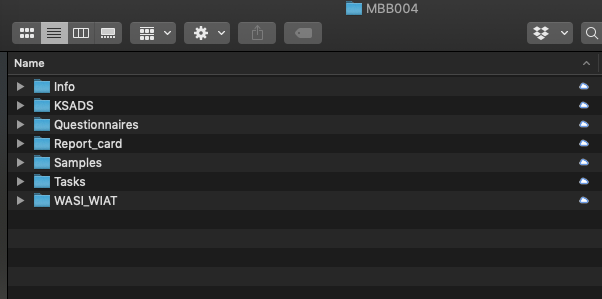
\includegraphics{images/final_checklist/report_cards/1.png}
\caption{}
\end{figure}

\begin{enumerate}
\def\labelenumi{\arabic{enumi}.}
\setcounter{enumi}{1}
\tightlist
\item
  Navigate to the report card folder and rename the template file - MBB999 to the relevant participant - and open the file
\end{enumerate}

\begin{figure}
\centering
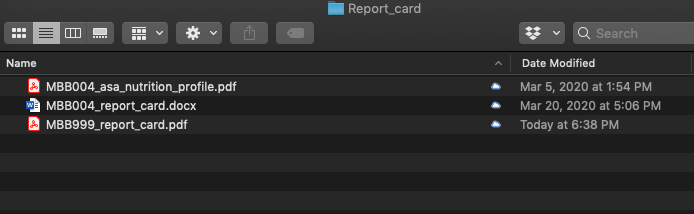
\includegraphics{images/final_checklist/report_cards/2.png}
\caption{}
\end{figure}

\begin{enumerate}
\def\labelenumi{\arabic{enumi}.}
\setcounter{enumi}{2}
\tightlist
\item
  If an ASA nutrition report has been generated for this participant, delete page 4 of the pdf. If no ASA nutrition report has been generated, delete page 3 of the pdf.
\end{enumerate}

\begin{figure}
\centering
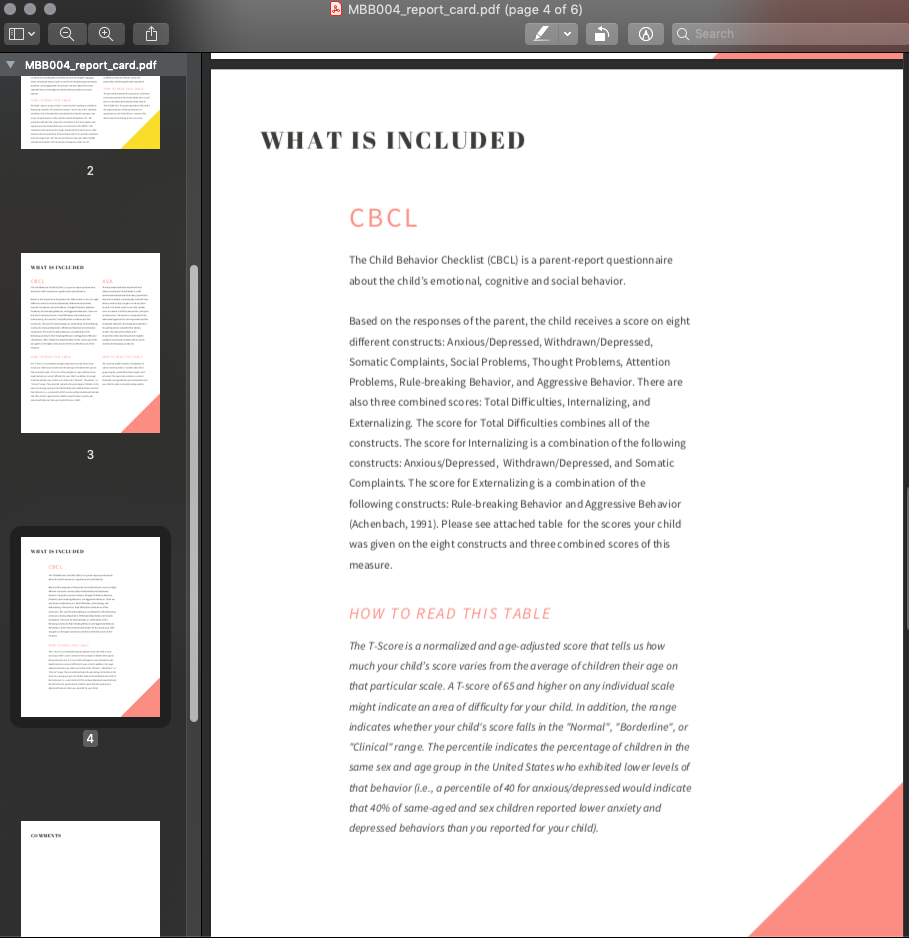
\includegraphics{images/final_checklist/report_cards/3.png}
\caption{}
\end{figure}

\begin{enumerate}
\def\labelenumi{\arabic{enumi}.}
\setcounter{enumi}{3}
\tightlist
\item
  Navigate to the last pge of the pdf, and fill in the scores for this participant. You can type directly on the page - it is a fillable form.
\end{enumerate}

\begin{figure}
\centering
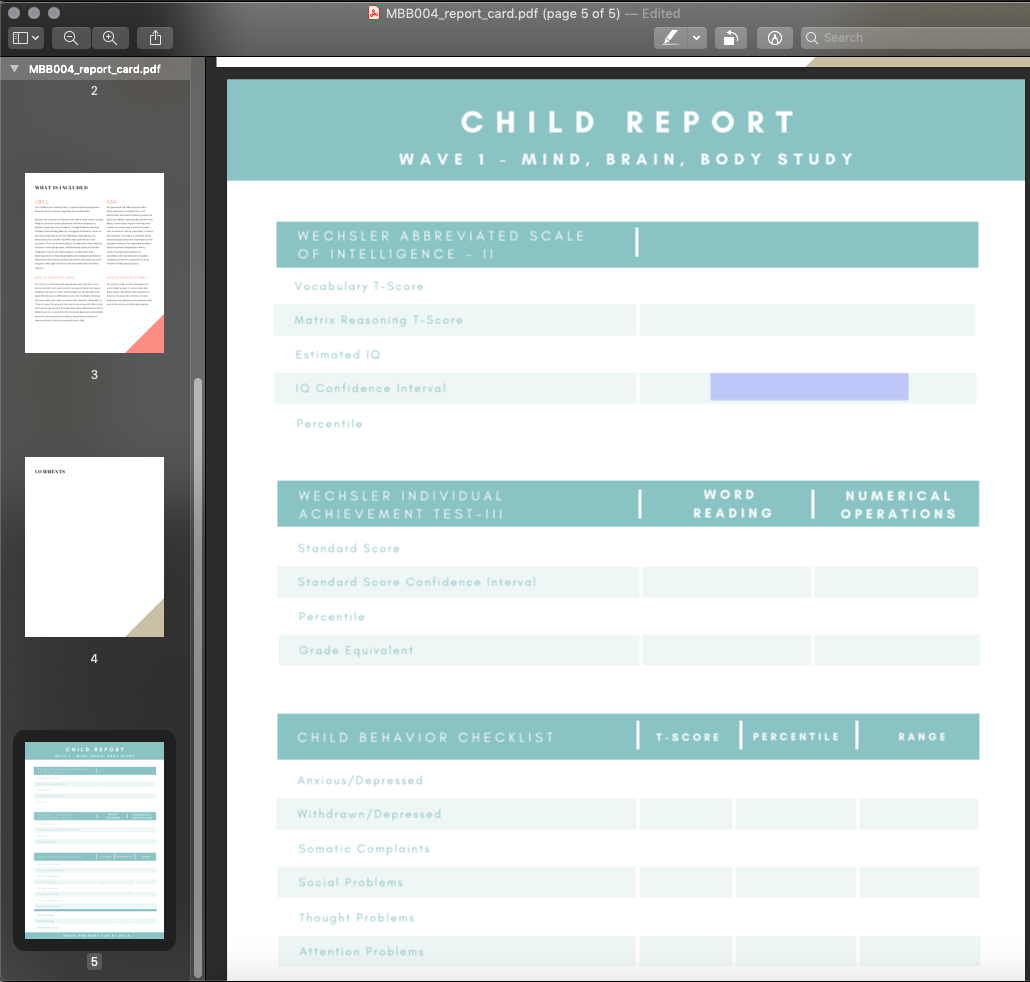
\includegraphics{images/final_checklist/report_cards/4.png}
\caption{}
\end{figure}

\begin{enumerate}
\def\labelenumi{\arabic{enumi}.}
\setcounter{enumi}{4}
\tightlist
\item
  After you have entered the data, it should look like this
\end{enumerate}

\begin{figure}
\centering
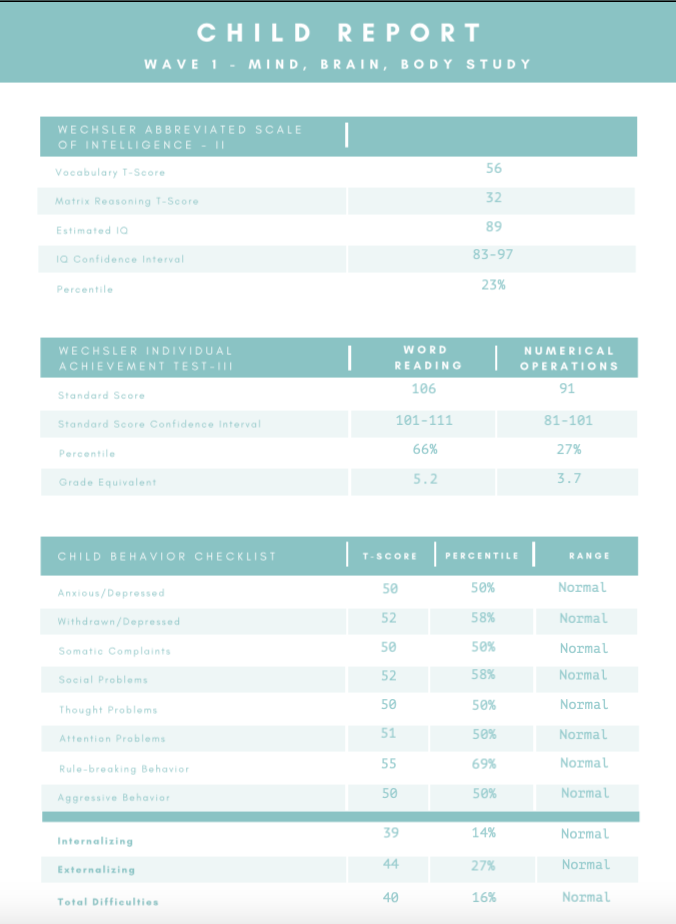
\includegraphics{images/final_checklist/report_cards/5.png}
\caption{}
\end{figure}

\begin{enumerate}
\def\labelenumi{\arabic{enumi}.}
\setcounter{enumi}{5}
\tightlist
\item
  If there are any comments, enter them on the comments page.
\end{enumerate}

\begin{itemize}
\item
  For example, if any NA's are present due to less than 70\% of data for that subset being available to calculate a score - note that here. Or, for example if the child was too young to receive a grade based score, you could note the aged based reading of the table here.
\item
  If there are no comments, delete this page.
\end{itemize}

\begin{figure}
\centering

\includegraphics{images/final_checklist/report_cards/6.png}
\caption{}
\end{figure}

\begin{enumerate}
\def\labelenumi{\arabic{enumi}.}
\setcounter{enumi}{6}
\tightlist
\item
  \textbf{Important} - Once you have completed the edits to the pdf, you must follow these steps to ``lock'' the data so that it is no longer editable before sending to the participant. To do so, click file/print/PDF/Save as PDF. Save the PDF to your desktop, then replace the original PDF with the desktop version.
\end{enumerate}

\begin{figure}
\centering
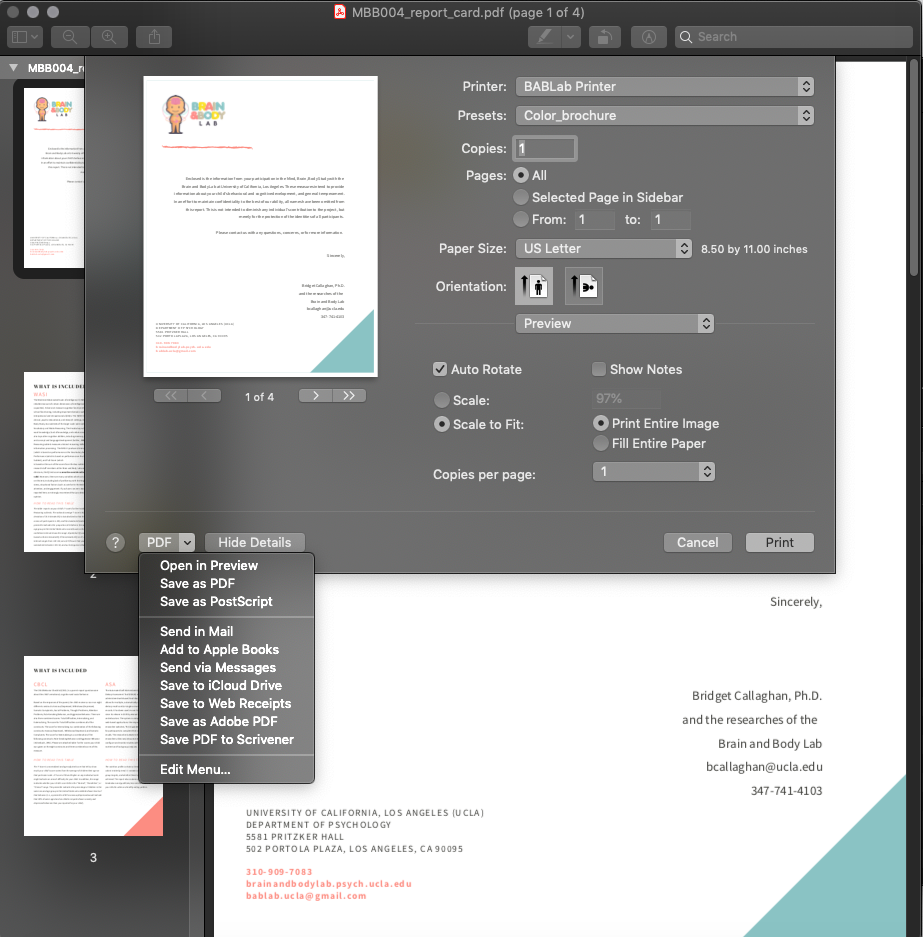
\includegraphics{images/final_checklist/report_cards/7.png}
\caption{}
\end{figure}

\begin{enumerate}
\def\labelenumi{\arabic{enumi}.}
\setcounter{enumi}{7}
\tightlist
\item
  The report card is now ready to be sent to the participant.
\end{enumerate}

\begin{center}\rule{0.5\linewidth}{\linethickness}\end{center}

\hypertarget{protocols}{%
\chapter{Protocols}\label{protocols}}

\hypertarget{consent}{%
\section{Consent}\label{consent}}

Once the parent and child come into the lab, seat them in the rainbow room on the couch for consenting.

Make some small talk - Ask the participant how they got here. If they have participated before in research. Offer them a bottle of water. Thank them for coming and for giving up their weekend to help science.

Tell the parent and child that the first thing you are going to do is go over all of the things they will do today, and have them sign the consent forms.

Speak to them and direct them through the whole process.

\hypertarget{things-you-will-do-in-the-lab}{%
\subsection{Things you will do in the lab}\label{things-you-will-do-in-the-lab}}

\begin{itemize}
\tightlist
\item
  Stick stickers on you to measure heart rate, sweat, stomach muscles.
\item
  Sit with parent and talk about fun things and hard things (filming).
\item
  Parent stays in room and answers more questions.
\item
  Child goes next door to play computer games (look at pictures, watch movies). Some of the movies and pictures will be a little bit scary, others sad, others boring.
\item
  One of the games involves a loud annoying noise, we will adjust it for you.
\item
  You will also do some other games on paper and pencil - like puzzle and word games
\item
  You will answer some questionnaires
\item
  We will also measure your height, weight, and waist circumference.
\item
  We will take three biological samples:

  \begin{itemize}
  \tightlist
  \item
    Hair - stress hormones
  \item
    Saliva - microbiome
  \item
    Blood - immune - wear goggles
  \end{itemize}
\item
  Do you get sick or dizzy when you see blood or hurt yourself?
\item
  If we need to, can we prick two fingers?
\item
  When you are done with all of that, you will get a big prize, then we will pay you and you will go home.
\item
  You will get \$45 for the work you put in today.
\end{itemize}

\hypertarget{things-you-will-do-at-home}{%
\subsection{Things you will do at home}\label{things-you-will-do-at-home}}

Child

\begin{itemize}
\tightlist
\item
  Poop sample - microbiome
\item
  Stool scale
\item
  Memory game - to see what you remember from lab.
\end{itemize}

Parent

\begin{itemize}
\tightlist
\item
  24 hour food recall
\end{itemize}

When you complete the poop sample and the games at home, we will pay you another \$20 in the form of a giftcard.

\hypertarget{things-to-know}{%
\subsection{Things to know}\label{things-to-know}}

You are a volunteer, which means that you do not have to do anything, or say anything that makes you uncomfortable. We would like you to try everything you can, and to do your best, but if there are things you absolutely do not want to do, just tell us, that is o.k.

We keep your participation confidential - ID number.

We want you to come in again in the future, so we will ask for some information so we can contact you in the future.

\emph{Sign consent/assent forms including DBS form and Contact Sheet}

\begin{center}\rule{0.5\linewidth}{\linethickness}\end{center}

\hypertarget{recruitment}{%
\section{Recruitment}\label{recruitment}}

\hypertarget{pre-screening}{%
\subsection{Pre-Screening}\label{pre-screening}}

\begin{enumerate}
\def\labelenumi{\arabic{enumi}.}
\tightlist
\item
  Check if participant is in Recruitment Database

  \begin{itemize}
  \tightlist
  \item
    If not, add them to the Recruitment Database
  \end{itemize}
\item
  Check if participant is in ID Drive

  \begin{itemize}
  \tightlist
  \item
    If yes, check if they have a Screener ID
  \item
    If not, assign them a Screener ID once contact has been established based on the next available Screener ID \# in REDCap and proceed with screening
  \item
    If yes, proceed with screening under existing Screener ID in REDCap
  \end{itemize}
\end{enumerate}

\hypertarget{screening}{%
\subsection{Screening}\label{screening}}

\begin{enumerate}
\def\labelenumi{\arabic{enumi}.}
\tightlist
\item
  To screen a new participant click ``Add / Edit Records''
\item
  Click to enter a new Subject ID

  \begin{itemize}
  \tightlist
  \item
    Make sure Arm 1: Recruitment is selected
  \end{itemize}
\item
  Type ``SMBB\#'' (Screener ID) to create a record and hit ``Enter''

  \begin{itemize}
  \tightlist
  \item
    Make sure to link the participants Screener ID and their name on the \textbf{ID Drive ONLY}
  \item
    Before creating a new record, be sure to check the ID Drive to see if the participant already has an existing Screener ID
  \item
    If a record exists, add a new instance of the screen instead of creating a new record
  \end{itemize}
\item
  The screening arm contains two parts

  \begin{itemize}
  \tightlist
  \item
    The screen
  \item
    The wave1\_status

    \begin{itemize}
    \tightlist
    \item
      The wave1\_status is to be updated after the first and each subsequent contact
    \end{itemize}
  \end{itemize}
\item
  Click on the radio button in the ``screen'' row to screen the participant
\item
  Click ``Now'' to enter today's date and time
\item
  Select the appropriate choice to start the phone call and follow the skip logic.
\item
  Follow the skip logic to the end.

  \begin{itemize}
  \tightlist
  \item
    For items without a text field, write the information down in the Recruitment database (This identifying information cannot be on REDCap)
  \end{itemize}
\item
  Once done, select ``Complete'' and ``Save \& Exit Form''

  \begin{itemize}
  \tightlist
  \item
    The screen can be entered multiple times - for instance if there are multiple phone calls or contacts
  \item
    It is important to keep a record of all instances of contact
  \end{itemize}
\item
  Click the screen\_status radio button
\item
  Select the appropriate option

  \begin{itemize}
  \tightlist
  \item
    Contact - Participant needs to be re-contacted (add Recruitment Database \& ID Drive)
  \item
    Ineligible - Participant not eligible for study
  \item
    To Enroll - Participant to enroll (need to create subject ID, enter subject info, schedule participant, add to Recruitment Database, add to ID Drive)
  \item
    Enrolled - Participant has been enrolled (all above have been completed)
  \item
    To Remove - Participant wants to be removed
  \end{itemize}
\item
  Be sure to update the screen status after each contact

  \begin{itemize}
  \tightlist
  \item
    After 3 contacts (with no response) - review (time of day, contact method, etc.)
  \end{itemize}
\item
  If enrolled, proceed to pre-session checklist in the participant log
\end{enumerate}

\hypertarget{other-screening-information}{%
\subsection{Other Screening Information}\label{other-screening-information}}

Accessing Lists

To find out where participants are in the recruitment process, there are several lists.

\begin{enumerate}
\def\labelenumi{\arabic{enumi}.}
\tightlist
\item
  Click on ``Record Status Dashboard''
\item
  Participants who have been enrolled will be listed in the Enrollment - Wave 1 list
\item
  Participants in the process of recruitment will be listed in one of the 4 Recruitment lists

  \begin{itemize}
  \tightlist
  \item
    *These lists are populated based on the individuals ``Screen Status'' so be sure to update after each contact!
  \end{itemize}
\end{enumerate}

List Types

\begin{itemize}
\tightlist
\item
  Contact - List of individuals who need to be contacted or re-contacted (also includes waitlist)
\item
  Ineligible - Participants are ineligible but interested
\item
  To Enroll - Participants who have been screened and are eligible to enroll
\item
  To Remove - Participants who were not interested in being contacted for this or future research
\end{itemize}

\hypertarget{addressing-concerns}{%
\section{Addressing Concerns}\label{addressing-concerns}}

If a parent has a concern about the study before the session, send the email template:

\begin{itemize}
\tightlist
\item
  {[}MBB - CONCERNS{]}
\end{itemize}

\begin{center}\rule{0.5\linewidth}{\linethickness}\end{center}

Callaghan, B. L., Fields, A., Gee, D. G., Gabard-Durnam, L., Caldera, C., Humphreys, K. L., Goff, B., Flannery, J., Telzer, E. H., Shapiro, M., \& Tottenham, N. (2020). Mind and gut: Associations between mood and gastrointestinal distress in children exposed to adversity. Development and Psychopathology, 32(1), 309--328. \url{https://doi.org/10.1017/S0954579419000087}

(Callaghan et al., 2020)

\citep{xie2015}

\citep{callaghanMindGutAssociations2020a}

\bibliography{book.bib,packages.bib}


\end{document}
